\chapter{The CMS Detector at the Large Hadron Collider}

The CMS detector is a general purpose particle detector that measures the energy and momentum of particles produced in the collision of high-energy protons in the Large Hadron Collider (LHC) at CERN \cite{collaborationCMSExperimentCERN2008}. It was designed with the goal of studying a wide range of physics phenomena, including the study of the electroweak sector, vector-boson scattering, precision studies of the standard model (SM), heavy-ion physics, and searches for physics beyond the SM. The CMS detector is cylindrical, with an overall diameter of $15.0 \text{ m}$, a length of $28.7 \text{ m}$ and a total width of $14,00\text{ m}$. A schematic of the CMS detector is shown in Figure \ref{fig:cms_detector}. Starting from the innermost subsystem of the detector, CMS is composed of the Silicon Tracker, the Electromagnetic and Hadron Calorimeters (ECAL and HCAL respectively), the super-conducting solenoid, and the muon system.

\begin{figure}[ht]
	\centering
	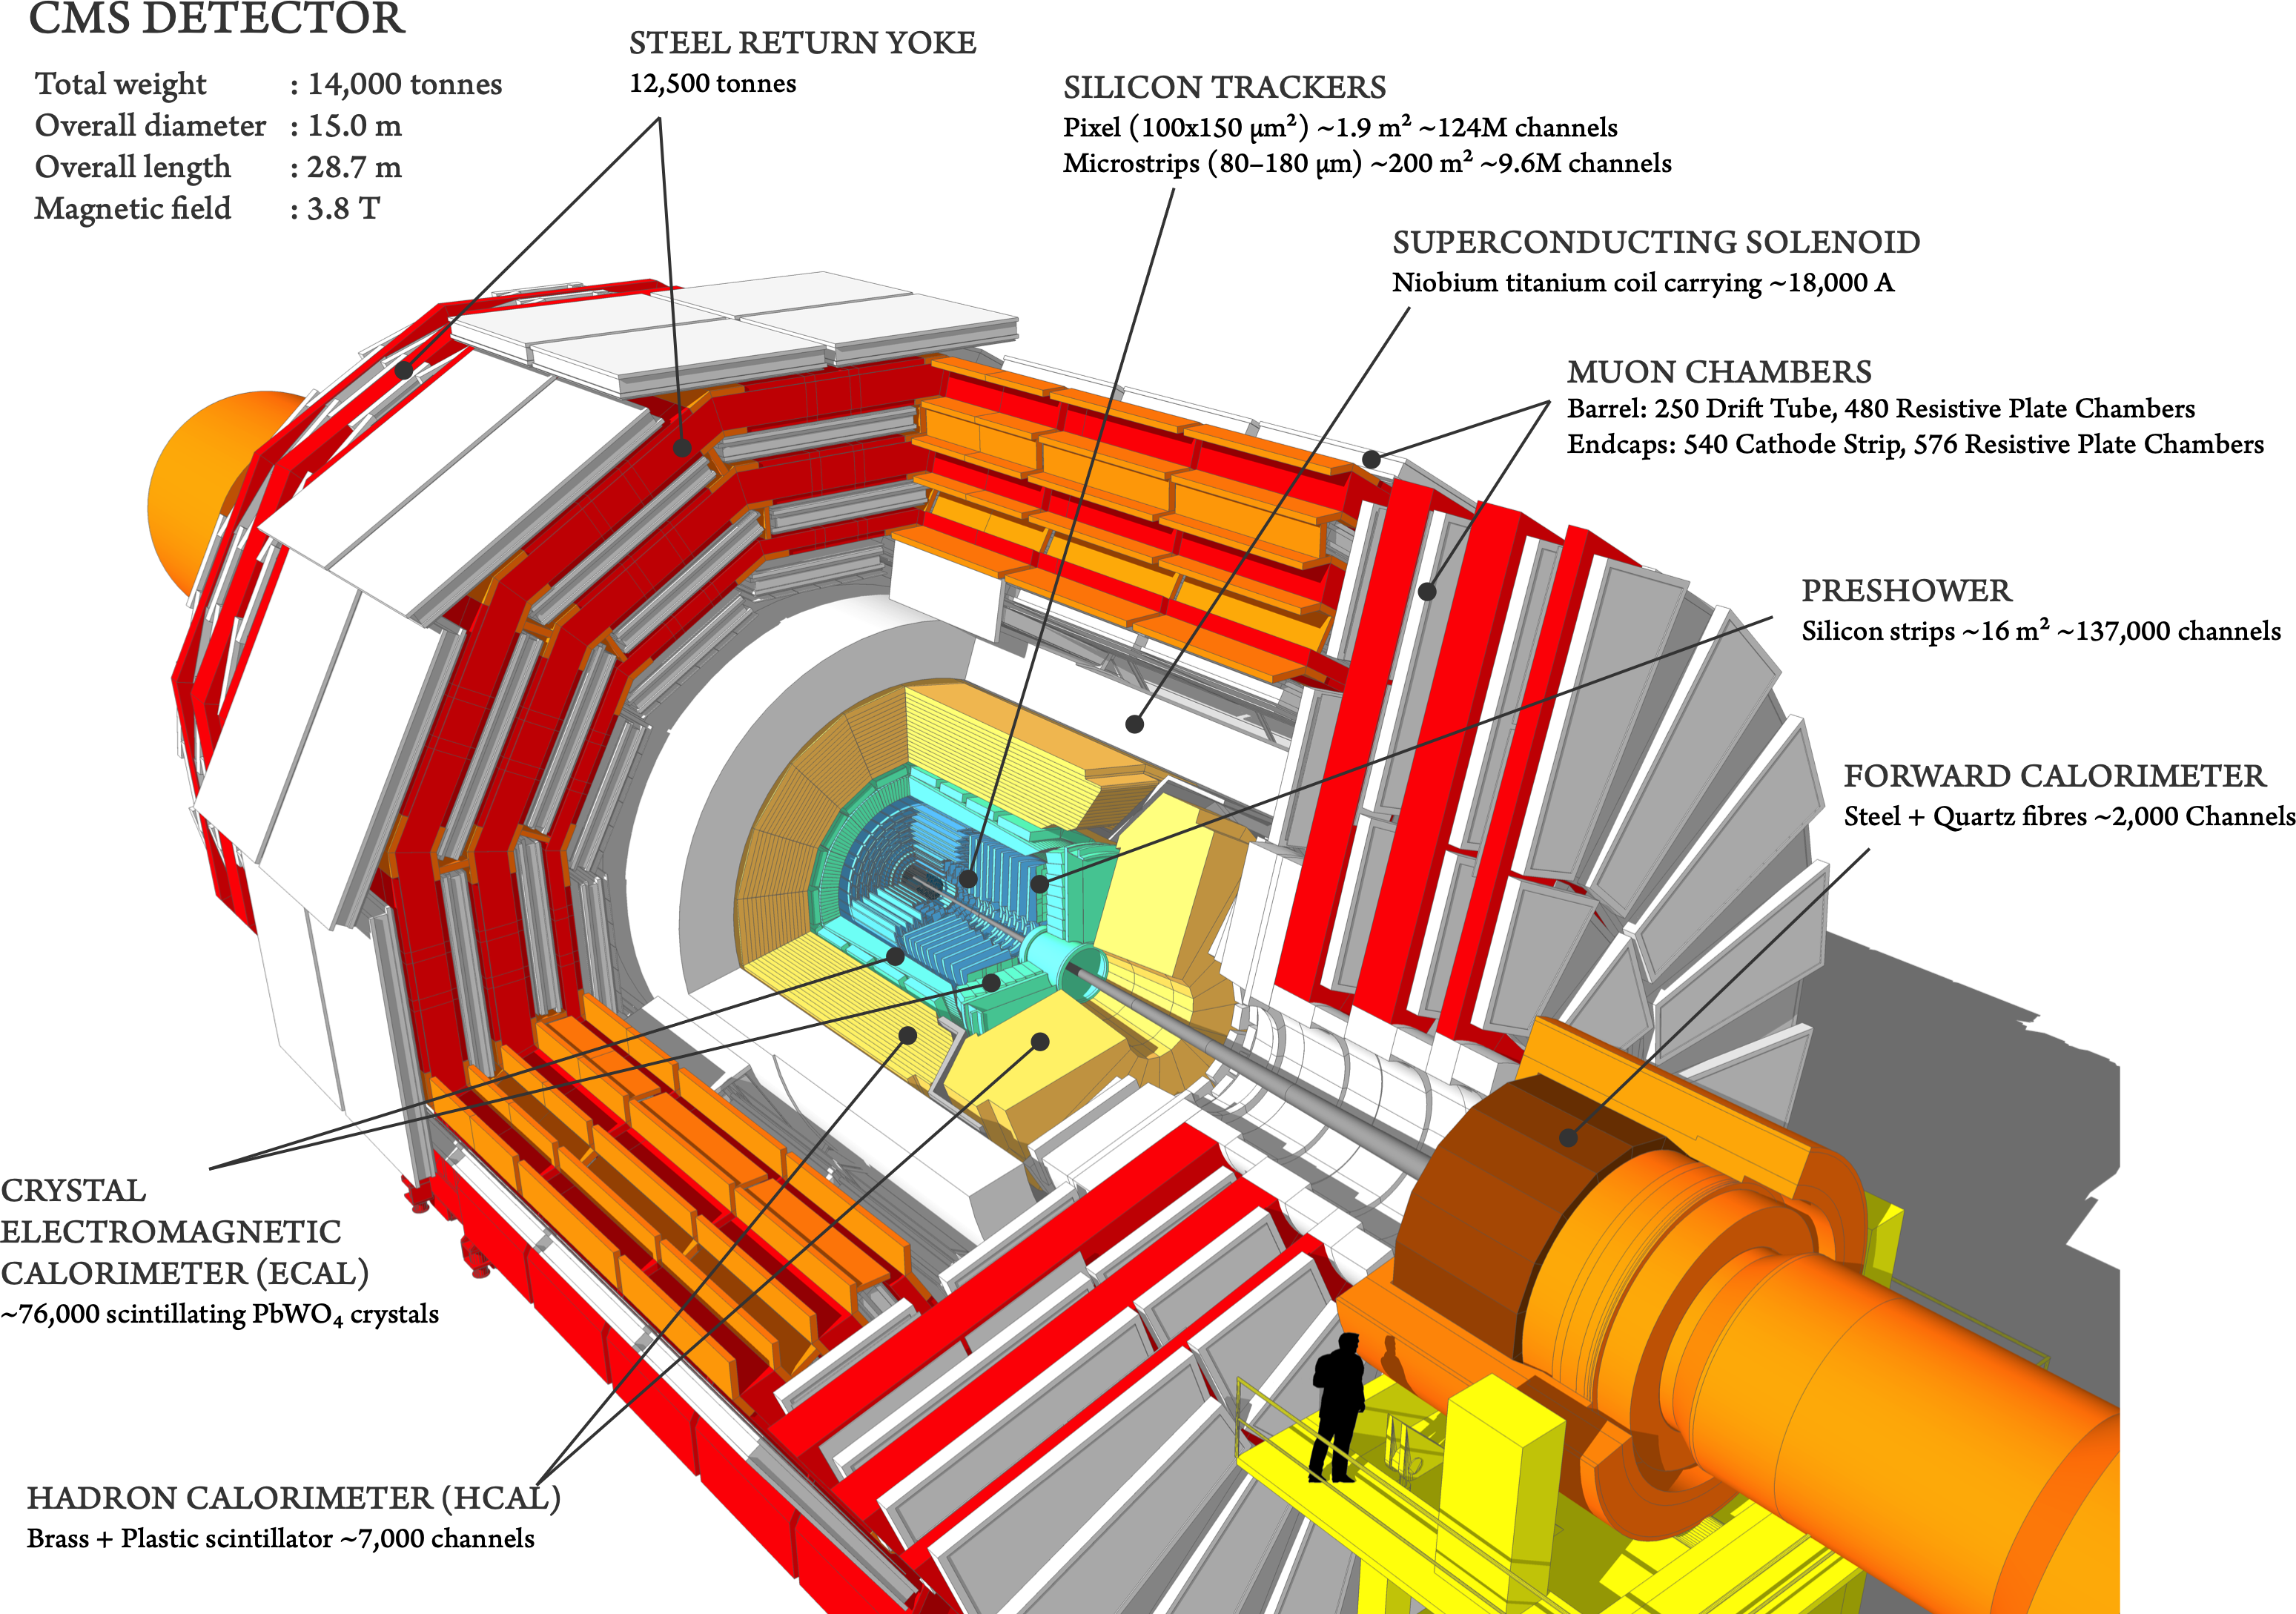
\includegraphics[width=0.8\textwidth]{images/cms_detector.png}
	\caption{Schematic of the CMS detector at the Large Hadron Collider.}
	\label{fig:cms_detector}
\end{figure}

% \section{Detector Overview}

% The CMS detector is one of the two large general-purpose detectors at the LHC located at CERN. Its overall length is of 

% Particular focus on the tracker and calorimeters. Should already include small discussion on Run 3 upgrades, particularly those things that enabled long-lived particle triggers.

% The Compact Muon Solenoid (CMS) detector is one of the two large general-purpose detectors at the Large Hadron Collider (LHC) located at CERN. It is designed to explore a wide range of physics, including the search for the Higgs boson, understanding the properties of the top quark, and searching for signs of physics beyond the Standard Model. The CMS detector is distinguished by its strong solenoidal magnetic field, which helps to bend the trajectories of charged particles, allowing for precise momentum measurements.
% At the heart of the CMS detector is the Tracker system, which is the innermost component. The Tracker is made up of pixel and strip detectors and is responsible for measuring the paths of charged particles as they pass through. This subsystem provides high-precision information about the trajectories of particles, helping to reconstruct their origins and contact points. The Tracker's ability to accurately determine the momentum of charged particles is crucial for a variety of physics analyses.
% Surrounding the Tracker, the CMS detector includes a sophisticated calorimetry system designed to measure the energy of particles. It is split into two parts: the Electromagnetic Calorimeter (ECAL) and the Hadronic Calorimeter (HCAL). The ECAL is composed of lead tungstate crystals that measure energy deposited by electrons and photons with high precision. The HCAL is located just outside the ECAL and is responsible for measuring the energy of more massive particles like hadrons. The combination of these calorimeters allows for full energy measurement of particles passing through the detector.
% The Muon system is another critical component of CMS, placed in the outermost layers of the detector. Muons, which are penetrating particles, can travel through dense materials with minimal attenuation, so they are detected in this outer subsystem. The Muon system uses several technologies, including drift tubes, cathode strip chambers, and resistive plate chambers to accurately track muon paths. It works in conjunction with the magnetic field to measure muon momentum and complements the information obtained from other subsystems to provide a comprehensive view of all particle interactions happening in a collision event.

\section{Silicon Tracker}

At the heart of the CMS detector is the Tracker system, which is the innermost subsystem. The Tracker is made up of pixel and strip detectors and is responsible for measuring the path of electrically charged particles. This subsystem was designed to offer high precision in the measurement of particle trajectories, allowing for an accurate reconstruction of the primary and secondary vertices. It offers excellent momentum resolution and track efficiency, allowing measurement of $p_{\text{T}}$ down to $50 \text{MeV}$ in the range of $|\eta| < 2.5$.

The tracker employs a two-layered structure:an inner section composed of silicon pixel layers, surrounded by a larger system of silicon strip layers with coarser segmentation. The sensors in both systems is made from doped silicon. When an energetic charged particles goes through a silicon sensor, it generates electron-hole pairs that drift in opposite directions within the semiconductor, producing a measurable current.

The current iteration of the pixel tracker features four barrel regions along with six endcap disks, providing a coverage of $|\eta| <2.5$. It was upgraded ahead of data-taking in 2017 in response to the increased instantaneous luminosities, increase readout bandwidth, computational load, and cumulative radiation damage.

Surrounding the pixel tracker, the silicon strip tracker is divided into an inner barrel, inner disks, outer barre, and outer endcaps. The strip sensors use a p-on-n doping structure and vary in thickness from $320 \;\mu\text{m}$ and $500 \;\mu\text{m}$. Compared to the pixel tracker, the strip sensors are significantly larger. Their dimensions range from $6\text{ cm} \times 12 \text{ cm}$ to $10\text{ cm} \times 9 \text{ cm}$. The full strip system comprises 34 layers (barrel and endcap combined, encompassing about $200 \text{ m}^2$ of silicon, and typically delivers nine or more spatial measurements per track with $|\eta|<2.4$.

Together, the pixel and strip detectors enable detailed tracking of charge particles. Around $|\eta| = 0$, the transverse impact parameter resolution is $10-100 \;\mu\text{m}$, while the longitudinal resolution is $40-140 \;\mu\text{m}$.

\section{Electromagnetic Calorimeter}

The electromagnetic calorimeter (ECAL) is designed to measure the energy of photons and particles with electric charge and it encloses the silicon tracker. It is composed of lead tungstate ($\text{PbWO}_4$) that scintillates when energetic charged particles pass through it, producing light which is detected by external photodetectors (avalanche photodiodes in the barrel and vacuum phototriodes in the endcaps). It is composed of a barrel and encap, both of which are composed of similarly shaped tapered prisms with square faces of $25 \text{ mm}$ by $28 \text{ mm}$, and $230 \text{ mm}$ in length. The barrel contains $61,200$ crystals, while the endcaps includes $14,648$.

A preshower detector is located in front of the ECAL endscaps. It enhances spatial resolution in the range $1.653 < |\eta| <2.6$ and it is composed of two lead layers, each followed by silicon strip sensors measuring $61\text{ mm} \times1.9\text{ mm}$, arranged in orthogonal directions.

\section{Hadronic Calorimeters}

The hadronic calorimeter (HCAL) is designed to measure the energy of particles, particularly hadrons, that are not entirely absored by the ECAL. It is composed of four main components: the hadron barrel (HB), hadron endcap (HE), hadron outer (HO) and hadron forward (HF) calorimeters. The HCAL's pseudorapidity span is $|\eta| <5.2$. As a sampling calorimeter, it has thick absorber layes to initiate particle showers and interleaved thin scintillating layers for energy detectionn and signal readout.

The HB covers a range of $|\eta| <1.3$ and extends radially from the outer edge of the ECAL to the inner boundary of the solenoid magnet. The absorber structure consists of fourteen layers cartridge brass, separated by structural steel plates, yielding $75 \text{ cm}$ of material. Between the brass layers, $3.7 \text{ mm}$ sheets of Kuraray SCSN-81 plastic scintillator are inserted, and an initial $9 \text{ mm}$ layers of Bicron BC408 scintillator is placed at the front. The resulting segmentation in both $\eta$ and $\phi$ is 0.087. The light emitted by the scincillators is captured by optical fibers and transmitted to hybrid photodiodes for detection.

The HE covers the angular region $1.3 <|\eta| < 3$. It has a similar configuration as the HB, with brass as the absorber material and SCSN-81 and BC408 scintillators as the active media. These are offset to ensure full spacial coverage.

The HO complements the HB by adding additional depth in the $|\eta| <1.3$ range, compensating for the radial space constraint imposed by the solenoid. It uses scintillator layers placed beyond the magnet, and the scintillator elements consist of 10 mm thick BC408 tiles, arranged with 0.087 granularity in $\eta$ and $\phi$, and read out via optical fiber.

The HF calorimeters extend the HCAL coverage to the forward region, spanning $3 <|\eta|<5.2$, and are located $11.2 \text{ m}$ from the interaction point. This region experiences a significantly higher particle flux compared to the rest of the HCAL components to particles with forward momentum, requiring greater radiation tolerance. The absorber consists of $165 \text{ cm}$ of steel. Quartz fibers generate Cherenkov radiation from charged particles within the shower. Half of the fibers are embedded starting $22 \text{ cm}$ from the detector's front to differentiate early EM showers from dee-penetrating hadronic ones, whereas the rest span the full detector length. These fibers are grouped into readout towers with segmentation $\Delta \eta \times \Delta \phi = 0.175\times0.175$, and the signal is detected using photomultiplier tubes.

\section{Muon System}

Muons, being heavier than electrons, have experience significantly lower Bremsstrahlung when traversing the material in the detector, and are thus less likely to be absorbed by the calorimeters and can even cross the solenoid. To account for this, there are three dedicated detectors within and surrounding the flux return yoke. These detectors are the drift tubes (DTs) in the barrel region, the cathode strip chambers (CSCs) in the endcaps, and the resistive plate chambers (RPCs) which are in both the endcaps and the barrel, make up the Muon system.

The three detector types in the Muon system operate under the same principle: a gas mixture is contained in an electric field and, when a muon traverses the gas, it ionizes the atoms, producing an electron cascade due to the high voltage ($3500 \text{ V}$ for DTs and CSCs, $9000 \text{ V}$ for RPCs).

There are a total of 250 DTs, providing a coverage of $|\eta| <1.2$. Each one features a central wire anode and a side cathode, with a rectangular cross-section of $13 \text{ mm}$ by $42 \text{ mm}$. They are layered in staggered formation and alternately oriented to obtain position measurements along the $r-\phi$ and $z$ axes. Based on drift time, the spatial resolution of a single DT is around $170 \;\mu\text{m}$, yielding an overall resolution of approximately $100 \;\mu\text{m}$ when combining multiple layers.

There are 468 CSCs which cover an interval of $0.9 <|\eta|< 2.4$. They


\section{Trigger System}

\section{Detector \& Data Quality Monitoring}

To ensure that the data from the CMS detector are of the utmost quality for the many physics analyses, there are Data Quality Monitoring (DQM) and Data Certification (DC) groups that monitor the health of the different subsystems of the CMS detector, as well as the integrity of the data. These groups conduct their monitoring during live data-taking (i.e., "online" operations) and also after the data have been fully reconstructed (i.e., "offline" operations). During Online DQM, live monitoring is performed on the status of the detector using quickly processed data in order to identify problems as soon as they appear. On the other hand, Offline DQM takes place hours afterward. During this second phase, experts evaluate a more thoroughly processed version of the same data seen in Online DQM, giving them access to more granular information on the performance of the detector and the quality of the physics reconstruction. Through this process, they provide certification flags that indicate whether or not the data pass the quality check for their particular subsystem and could be used for physics analysis. In addition, Offline experts can provide feedback to the Online crew of issues which they might have missed.

The data in both Online and Offline DQM is visualized through a platform dubbed DQMGUI (DQM Graphical User Interface). A screen capture showing an example run (run number 380238) is shown in Figure \ref{fig:dqmgui}. This platform shows a large collection of different plots and histograms, named monitoring elements, each showcasing a particular aspect of the detector (e.g., number of read-out chips in the Pixel detector) or physics reconstruction (e.g., track $p_T$ distributions). The data shown in these monitoring elements constitute a summary of what occurred during a given run, where a run is a continuous data-taking time period with particular data-taking conditions. These runs can be further subdivided into lumisections (LSs), which are periods of 23.3 seconds of data taking. Thus, most monitoring histograms result from the integration of the data over all LSs of the run, which can be made up of upwards of \~2000 LSs for the longest runs.

\begin{figure}
    \centering
    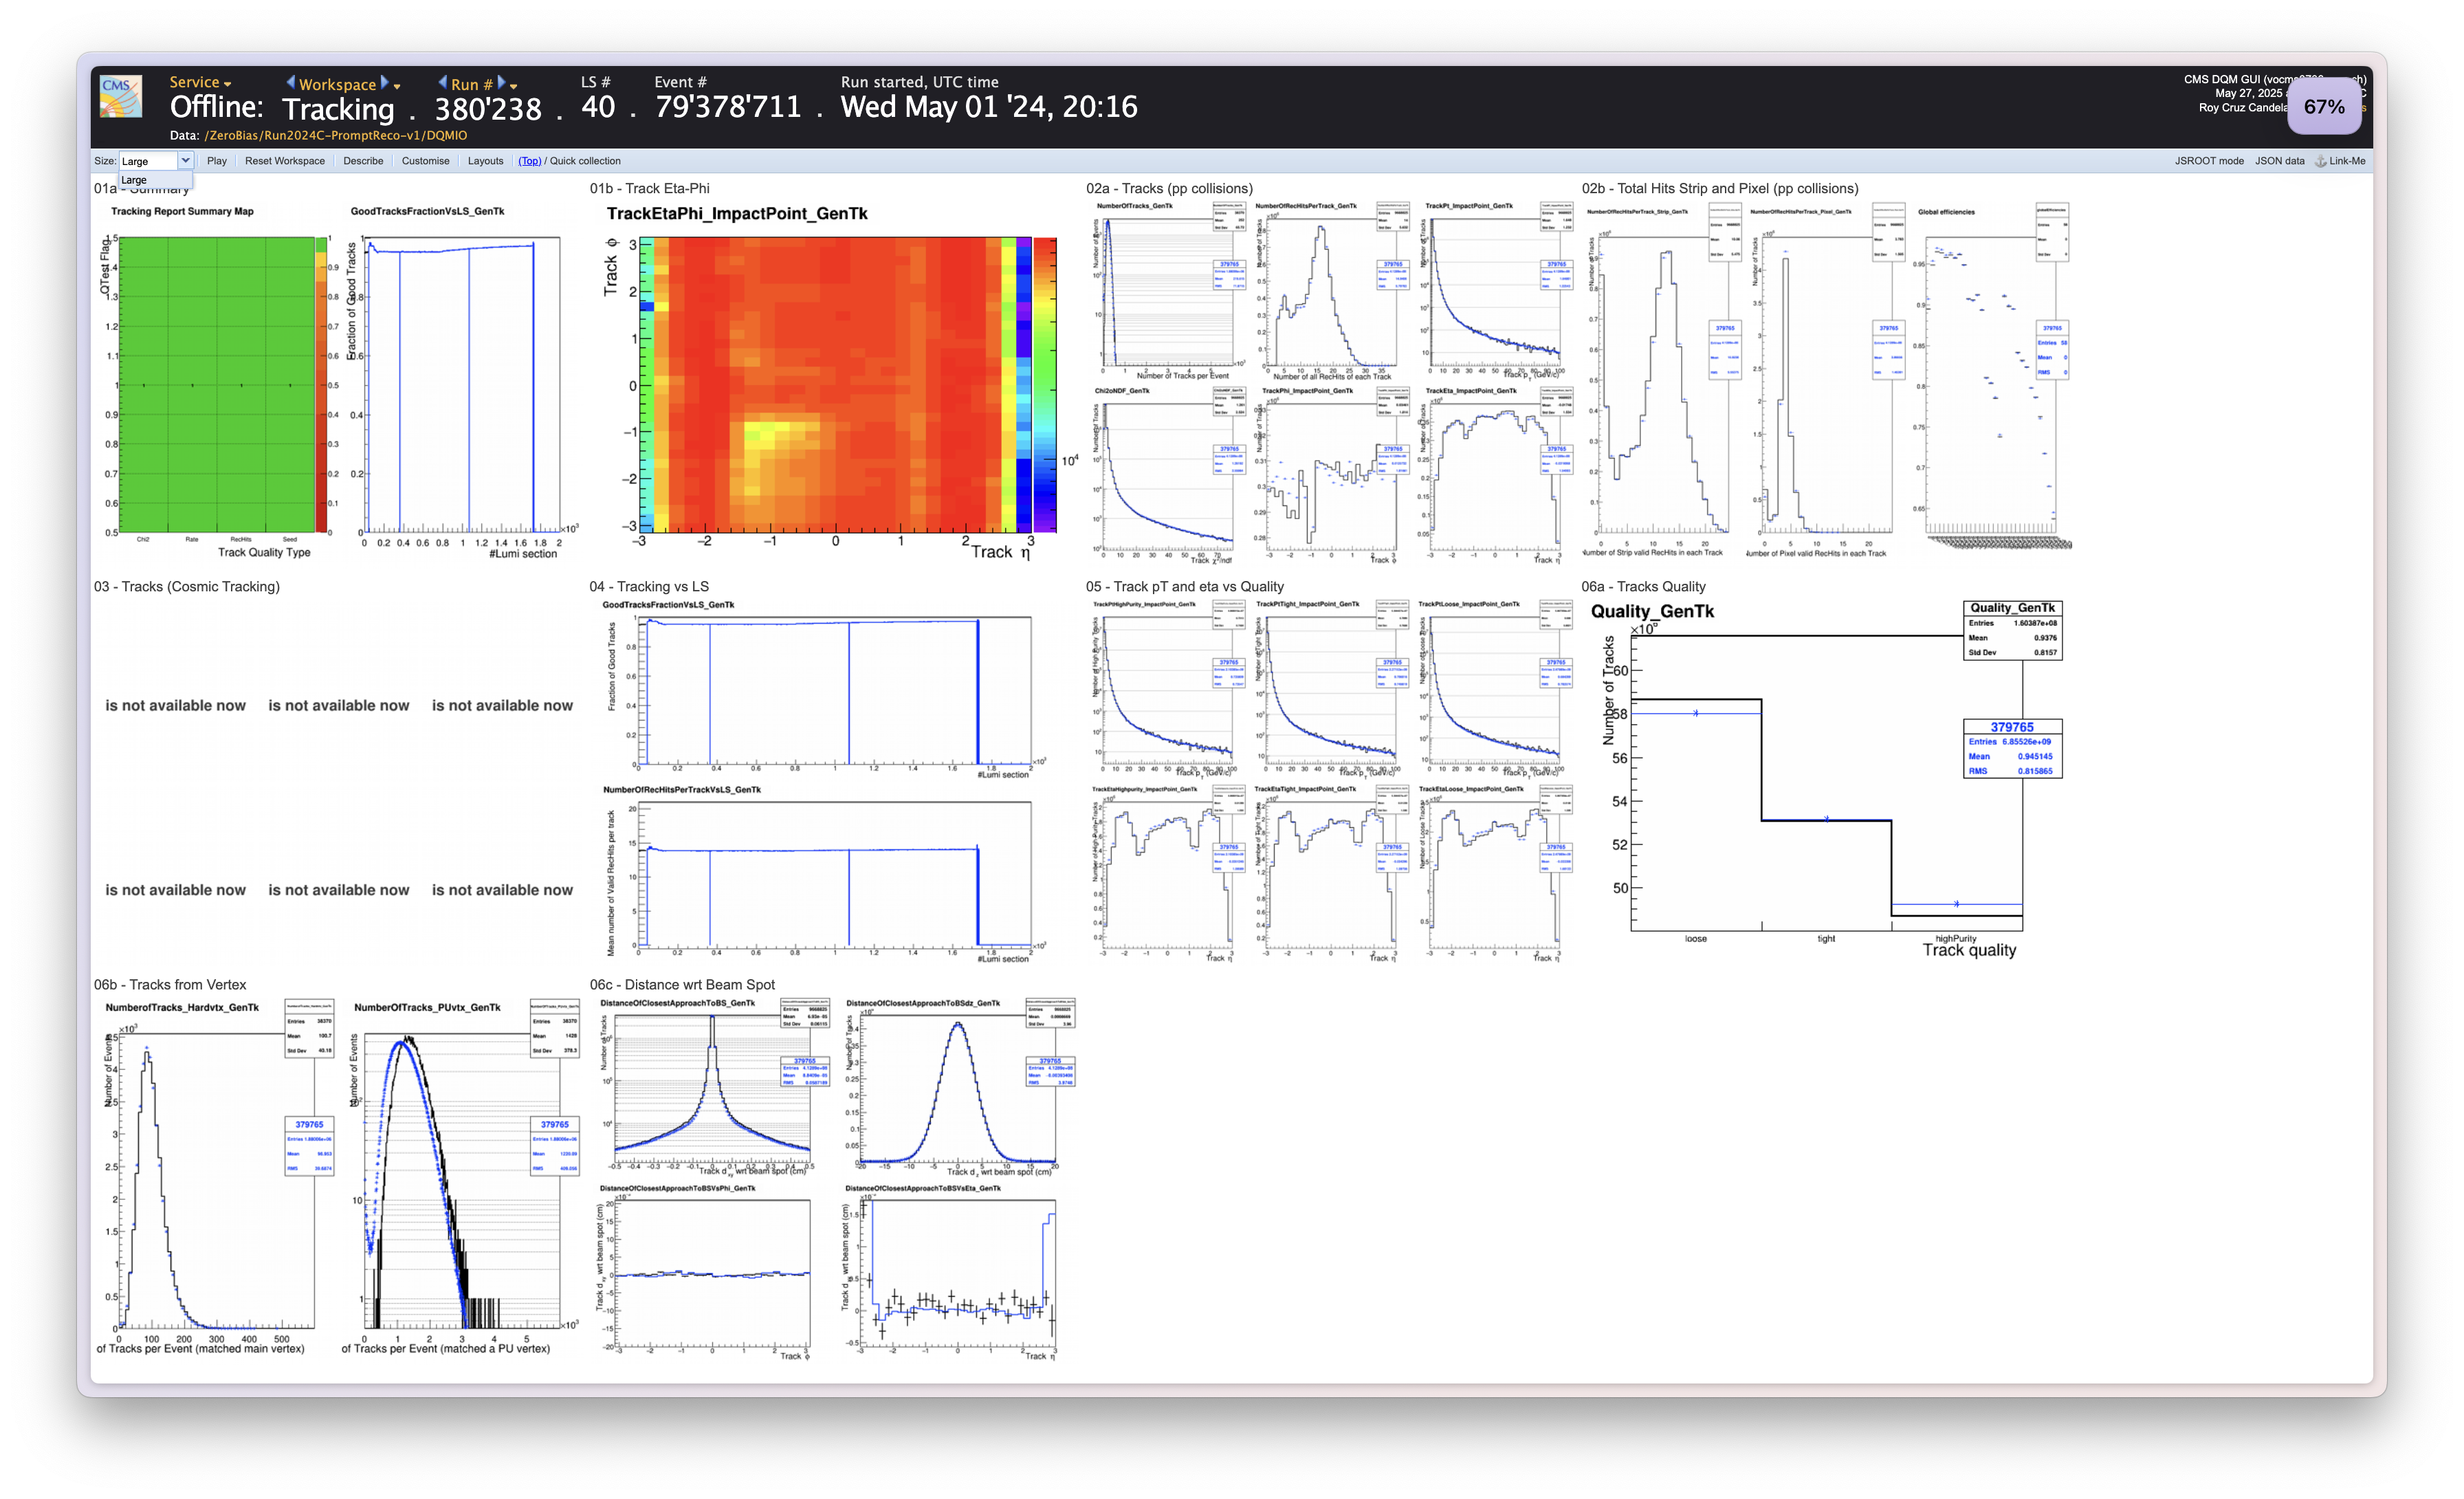
\includegraphics[width=0.8\linewidth]{images/dqmgui.png}
    \caption{Capture of example visualization of run 380238 in the DQMGUI}
    \label{fig:dqmgui}
\end{figure}